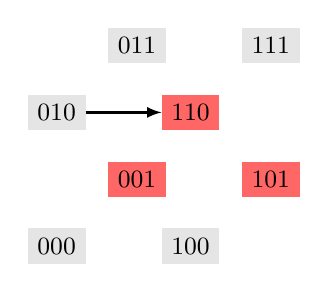
\begin{tikzpicture}
	\tikzstyle{stgstate} = [draw,shape=rectangle,font=\small, fill, color=gray!20]
	\tikzstyle{stgedge} = [-latex, thick,font=\sffamily\normalsize\bfseries]

	\def\incx{1.7}
	\def\incy{1.7}
	\colorlet{darkgreen}{green!50!black}

	% NODES %
	\node[stgstate] (000) at (0*\incx,0*\incy) {\textcolor{black}{000}};
	\node[stgstate] (100) at (1*\incx,0*\incy) {\textcolor{black}{100}};
	\node[draw,shape=rectangle,font=\small, fill, color=red!60] (001) at (0.6*\incx,0.5*\incy) {\textcolor{black}{001}};
	\node[draw,shape=rectangle,font=\small, fill, color=red!60] (101) at (1.6*\incx,0.5*\incy) {\textcolor{black}{101}};

	\node[stgstate] (010) at (0*\incx,1*\incy) {\textcolor{black}{010}};
	\node[draw,shape=rectangle,font=\small, fill, color=red!60] (110) at (1*\incx,1*\incy) {\textcolor{black}{110}};
	\node[stgstate] (011) at (0.6*\incx,1.5*\incy) {\textcolor{black}{011}};
	\node[stgstate] (111) at (1.6*\incx,1.5*\incy) {\textcolor{black}{111}};

	% EDGES %
	%g1
	\draw[stgedge] (010) edge (110);
	%g2
	\end{tikzpicture}
